\documentclass{article}
\usepackage{joyce-math, joyce-bib, joyce-graphics}
\bibpunct{(}{)}{;}{a}{,}{,}
\begin{document}

\section{Demonstrating Improved Accuracy}

We have gone to considerable trouble to develop our skew-normal approximation
for the binomial; now comes the time to justify our efforts by demonstrating
its improved accuracy over the regular normal one.

\subsection{Visual Comparison}

The first, and most obvious, way of judging accuracy is by visual inspection.
Figures \ref{fig:comparison-n25}, \ref{fig:comparison-n50}, and
\ref{fig:comparison-n100} compare the binomial, normal, and skew-normal at
small values of $p$ for $n=25$, $n=50$, and $n=100$, respectively. It is not
hard to see that, especially at very small $n$ and $p$, our skew-normal curve
follows the shape of the binomial much more accurately.

\begin{figure}[h]
  \centering
  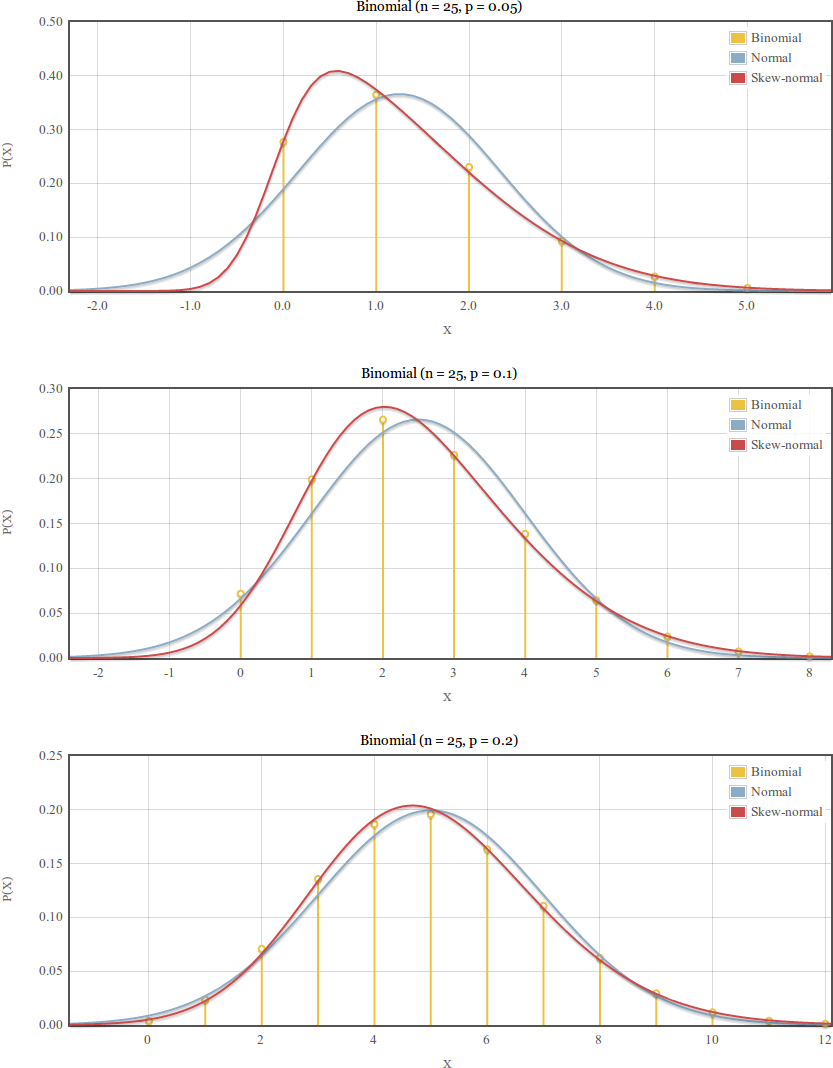
\includegraphics[width=\textwidth]{../graphs/images/comparison-n25.png}
  \caption{Binomial, normal, and skew-normal, $n=25$}
  \label{fig:comparison-n25}
\end{figure}

\begin{figure}[h]
  \centering
  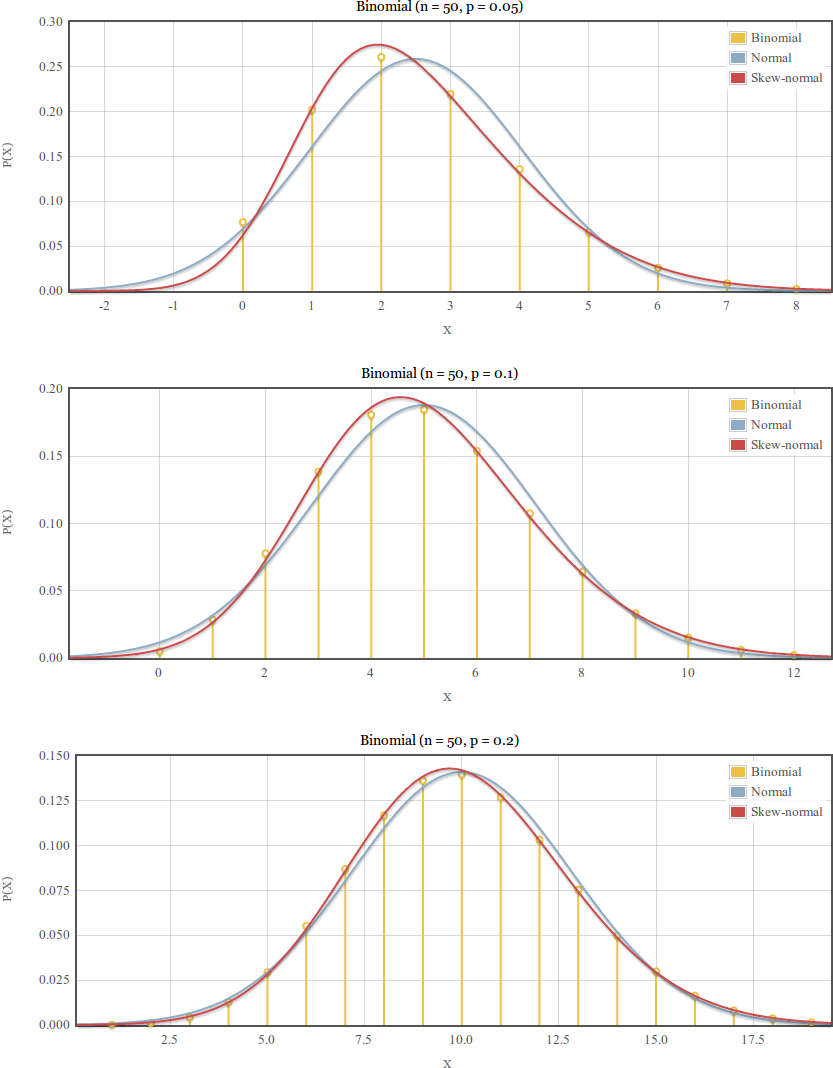
\includegraphics[width=\textwidth]{../graphs/images/comparison-n50.png}
  \caption{Binomial, normal, and skew-normal, $n=50$}
  \label{fig:comparison-n50}
\end{figure}

\begin{figure}[h]
  \centering
  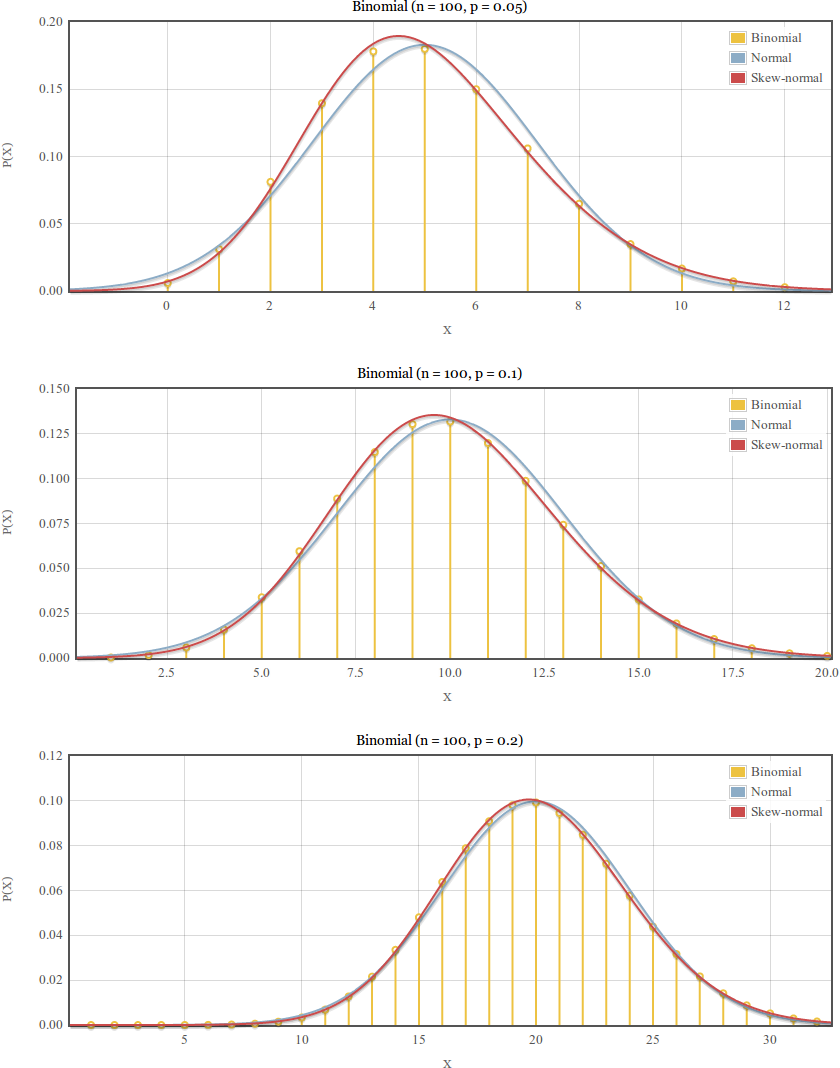
\includegraphics[width=\textwidth]{../graphs/images/comparison-n100.png}
  \caption{Binomial, normal, and skew-normal, $n=100$}
  \label{fig:comparison-n100}
\end{figure}

\subsection{Maximal Absolute Error}

Another more numerical method would be to compare the maximal absolute errors
of our two approximations, defined by \citet{mabs} as

\begin{equation}
  \textnormal{MABS}(n, p) \eq \max_{k \in \{0, 1,...,n\}} \left| F_{B(n,p)} (k) -  F_{\textnormal{appr}(n,p)}(k + 0.5) \right|
\end{equation}

where $F_{B(n,p)}$ is the cdf of the binomial and $F_{\textnormal{appr}(n,p)}$
is the cdf of either the normal or skew-normal approximation; the 0.5 is a
continuity correction.

Figure \ref{fig:mabs-fixed-n} shows the MABS as a function of $p$, for $n=25$
and $n=100$. Figure \ref{fig:mabs-fixed-p}, on the other hand, shows the MABS
as a function of $n$, for $p=0.05$ and $p=0.1$. Again, the skew-normal
outperforms the normal considerably in the extreme ranges, with the two
approximations converging as $n \rightarrow \infty$ or $p \rightarrow 0.5$.

\begin{figure}[h]
  \centering
  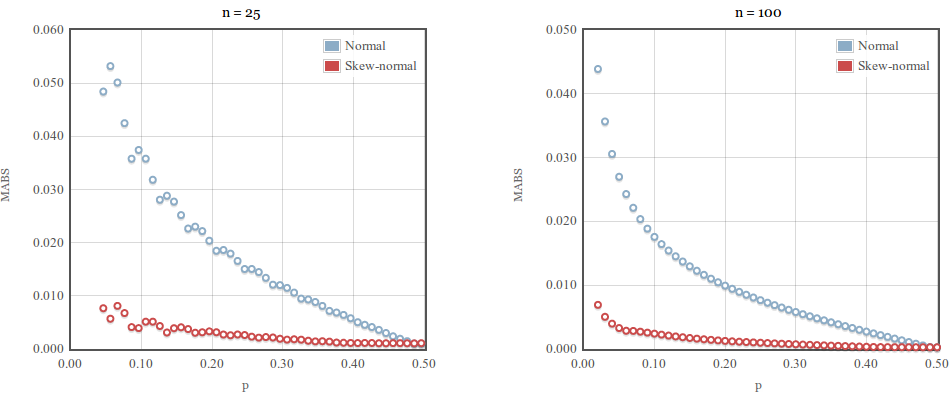
\includegraphics[width=\textwidth]{../graphs/images/mabs-fixed-n.png}
  \caption{MABS as a function of p}
  \label{fig:mabs-fixed-n}
\end{figure}

\begin{figure}[h]
  \centering
  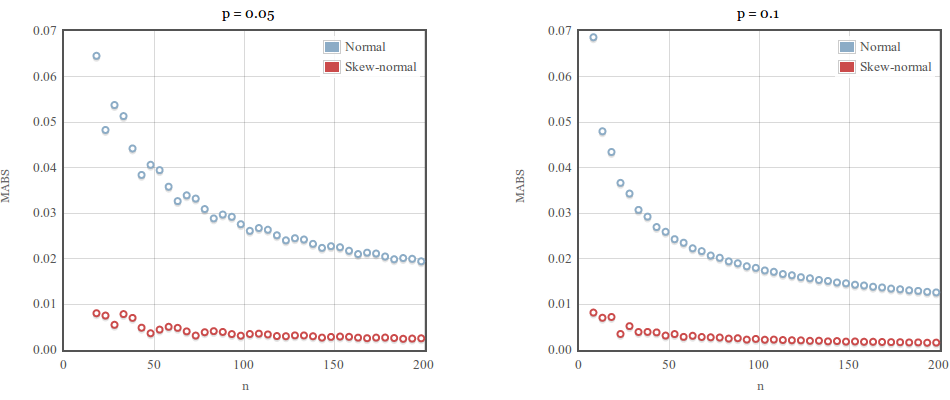
\includegraphics[width=\textwidth]{../graphs/images/mabs-fixed-p.png}
  \caption{MABS as a function of n}
  \label{fig:mabs-fixed-p}
\end{figure}

\nocite{*}

\bibliography{/home/joycetipping/projects/capstone/pieces/bibliography/bibliography.bib}
\bibliographystyle{plainnat}
\end{document}
